% TLDR: ICML 2026 Math-AI workshop poster (61x91 cm portrait, Stanford gemini theme, XeLaTeX)
% for "CertJudge: Evaluating Lean Formal-Code With Falsifiable Properties". Single canonical
% poster (visual-minimal style), reused across both workshop submissions.
% Compile: latexmk -xelatex -interaction=nonstopmode main.tex

\documentclass[final]{beamer}

% ====================
% Packages
% ====================

\usepackage[T1]{fontenc}
\usepackage{lmodern}
% Same sheet size as main.tex; scale bumped 1.0 -> 1.1 (less text, larger fonts for walk-by read).
\usepackage[size=custom,width=61,height=91,scale=1.1]{beamerposter}
\usetheme{gemini}
\usecolortheme{stanford}
% Highlighted (alert) blocks: cardinal title bar + faint red body so the two key
% blocks pop for the walk-by reader (stanford color theme leaves these unset).
\setbeamercolor{block alerted title}{fg=white,bg=cardinalred}
\setbeamercolor{block alerted separator}{bg=cardinalred}
\setbeamercolor{block alerted body}{fg=black,bg=cardinalred!7}
% Title one step down (\Huge -> \huge): with scale=1.1 this matches Draft A's visual size
% and keeps the long title on 2 lines instead of 3.
\setbeamerfont{headline title}{size=\huge,series=\bfseries}
\usepackage{amsmath}
\usepackage{graphicx}
\usepackage{booktabs}
\usepackage{tikz}
\usepackage{qrcode}

% ====================
% Lengths
% ====================
% (N+1)*\sepwidth + N*\colwidth = \paperwidth ; portrait 2-column: 3*0.03 + 2*0.455 = 1.0
\newlength{\sepwidth}
\newlength{\colwidth}
\setlength{\sepwidth}{0.03\paperwidth}
\setlength{\colwidth}{0.455\paperwidth}

\newcommand{\separatorcolumn}{\begin{column}{\sepwidth}\end{column}}
\newcommand{\tivar}{\ensuremath{\mathrm{TI}_{\mathrm{var}}}}

% ====================
% Title / authors
% ====================

\title{CertJudge: Evaluating Lean Formal-Code With Falsifiable Properties}

\author{Ethan S.~Hersch\inst{\normalsize *,1,\dag} \and Brando Miranda\inst{\normalsize *,1,\dag} \and Elyas Obbad~\inst{1} \and Srivatsava Daruru~\inst{1} \and Kirill Acharya~\inst{1,\dag} \and Zixiao Jolene Wang~\inst{2} \and Zhanke Zhou~\inst{3} \and Steven Dillmann~\inst{1} \and Yegor Denisov-Blanch~\inst{1} \and Sanmi Koyejo~\inst{1}}
\institute[Stanford]{\inst{1} Stanford University \qquad \inst{2} Harvard University \qquad \inst{3} Hong Kong Baptist University \\[0.5ex] \inst{\dag} Correspondence: \texttt{ehersch@stanford.edu, brando9@stanford.edu, kacharya@stanford.edu}}

% ====================
% Logo (reserves headline space so the title stays clear of it)
% ====================

\logoleft{
\includegraphics[height=5.5cm]{logos/icml_icon_only.png}}
\logoright{
\includegraphics[height=5.5cm]{stanford_logos/Block_S_2_color.png}}

% ====================
% Body
% ====================

\begin{document}

\begin{frame}[t]
\begin{columns}[t]
\separatorcolumn

% ============================================================
% LEFT COLUMN — hook, key idea, method (money figure carries it)
% ============================================================
\begin{column}{\colwidth}

  % CS197 moves 1-2: motivation folded into the single italic hook line
  \begin{block}{Validating LLM judges one human study at a time does not scale}

    {\centering\itshape Agents write Lean~4 code and its specs faster than humans can inspect --- can one human calibration, via automatic falsifiable checks, be amortized across every future judge?\par}

  \end{block}

  % CS197 move 3: the flip — certify with falsifiable behavioral checks instead of re-labeling
  \begin{alertblock}{Key idea: certify the judge --- don't re-label it}

    \begin{itemize}
      \setlength{\leftmargini}{2.2em}
      \setlength{\itemsep}{1.2ex}
      \item \textbf{CertJudge}: rate a small panel \textbf{once}.
      \item \textbf{Automatic falsifiable property checks} + \tivar{} certify every new judge --- no new labels.
      \item Calibration: $n{=}75$ candidate--gold Lean pairs, single annotator, two rubric passes; 8 judge configs per family panel.
    \end{itemize}

  \end{alertblock}

  % CS197 move 4: method/system — money figure, set larger than Draft A (0.86 -> 1.0 linewidth)
  \begin{block}{Four falsifiable properties in a trust index}

    \begin{figure}
      \centering
      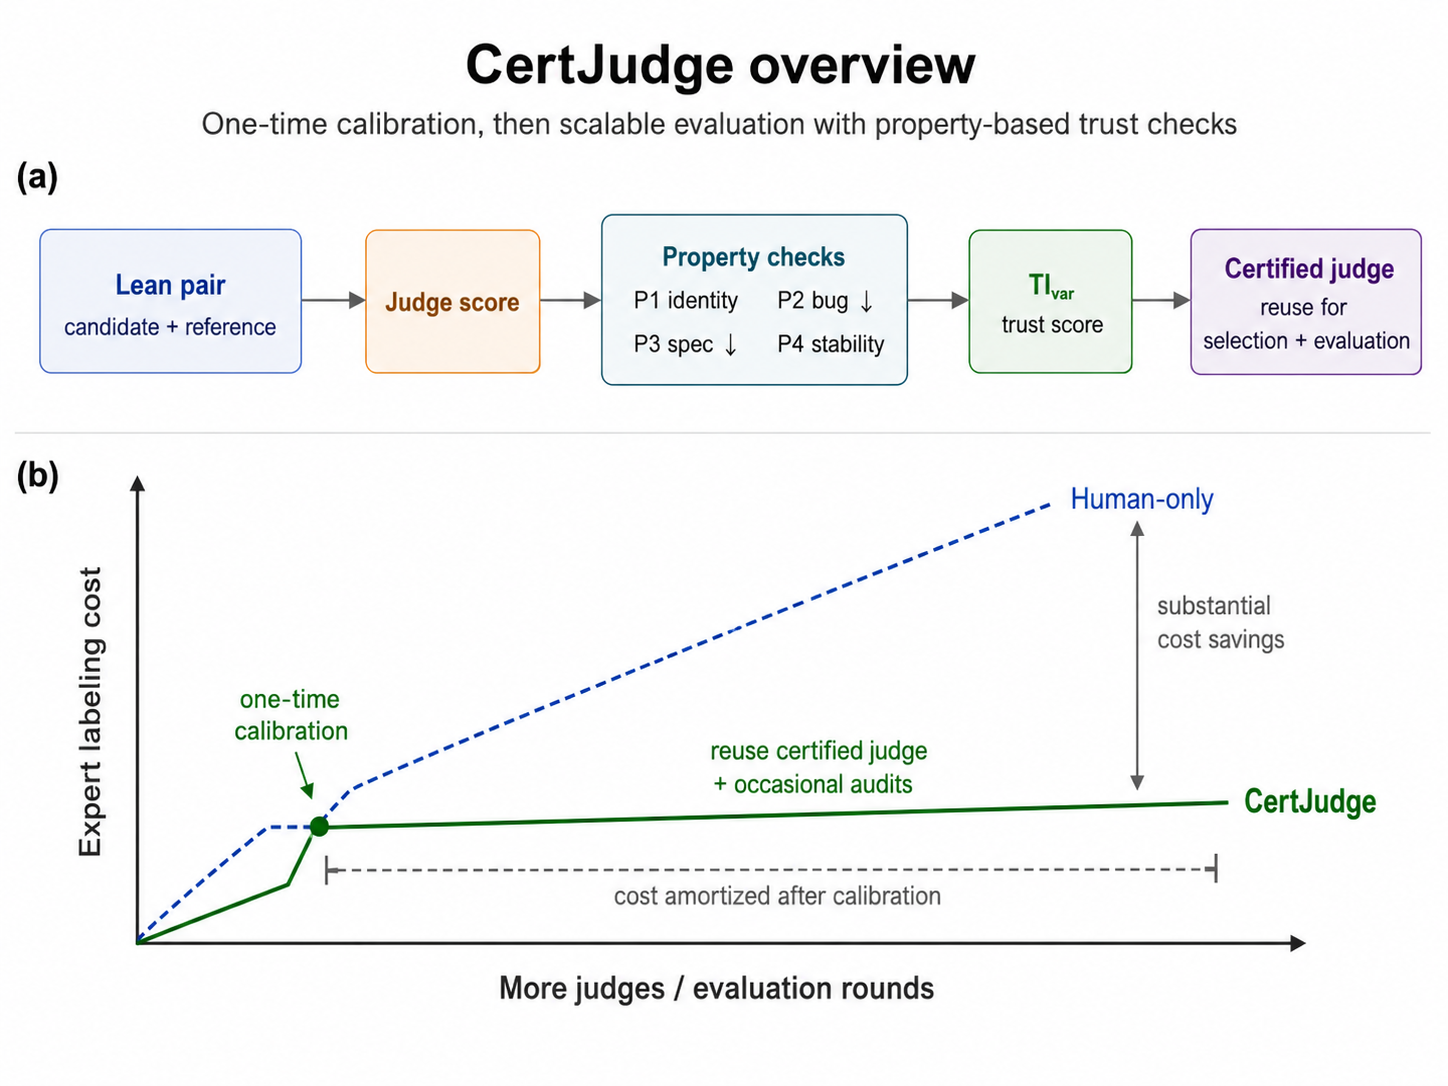
\includegraphics[width=\linewidth]{figures/pull_fig.png}
      \caption{Label once, then certify automatically --- labeling cost stops growing with the number of judges.}
    \end{figure}

    % P1-P4 as a 2x2 mini-grid, one phrase each (\tabularnewline keeps \raggedright safe in p-cells)
    \begin{center}
    \renewcommand{\arraystretch}{1.2}
    \begin{tabular}{@{}p{0.46\linewidth}@{\hspace{0.03\linewidth}}p{0.49\linewidth}@{}}
      \raggedright\textbf{P1 Identity:} $s(X,X)=1$ & \raggedright\textbf{P2 Bug monotonicity:} score $\downarrow$ as bugs injected \tabularnewline[1.0ex]
      \raggedright\textbf{P3 Spec monotonicity:} score $\downarrow$ as specs removed & \raggedright\textbf{P4 Stability:} invariant across repeats \& rewrites \tabularnewline
    \end{tabular}
    \end{center}

    \[
      \tivar = \exp\!\Big(
      \tfrac{1}{3}\log C_f
      + \tfrac{1}{3}\log(1-\widetilde{\mathrm{VarCorr}})
      + \tfrac{1}{3}\log(1-\widetilde{\mathrm{VarScore}})
      \Big)
    \]

    \begin{itemize}
      \setlength{\leftmargini}{2.2em}
      \item $C_f$ aggregates P1--P4 into a single geometric-mean score.
      \item \textbf{One failed property collapses the index.}
    \end{itemize}

  \end{block}

  % References moved from the right column to rebalance (right carries results + takeaways)
  \begin{block}{References}

    % Draft B keeps 3 entries (drops G-Eval); VeriBench is cited in the stress-test caption
    \nocite{Zheng2023MTBench,TongZhang2024CodeJudge}
    \footnotesize{\bibliographystyle{plain}\bibliography{poster}}

  \end{block}

\end{column}

\separatorcolumn

% ============================================================
% RIGHT COLUMN — results, takeaways, references
% ============================================================
\begin{column}{\colwidth}

  % CS197 move 5: headline result — big number + the ONE alignment visual
  \begin{block}{Result: \tivar{} predicts judge-level human alignment}

    \vspace{0.8cm}
    {\centering
      {\Huge $\boldsymbol{\rho = 0.833}$}\\[1.6ex]
      validation-set Spearman between \tivar{} and human agreement\\
      {\small avg labels; $0.905$ pass1 / $0.738$ pass2}\par
    }
    \vspace{0.4cm}

    \begin{figure}
      \centering
      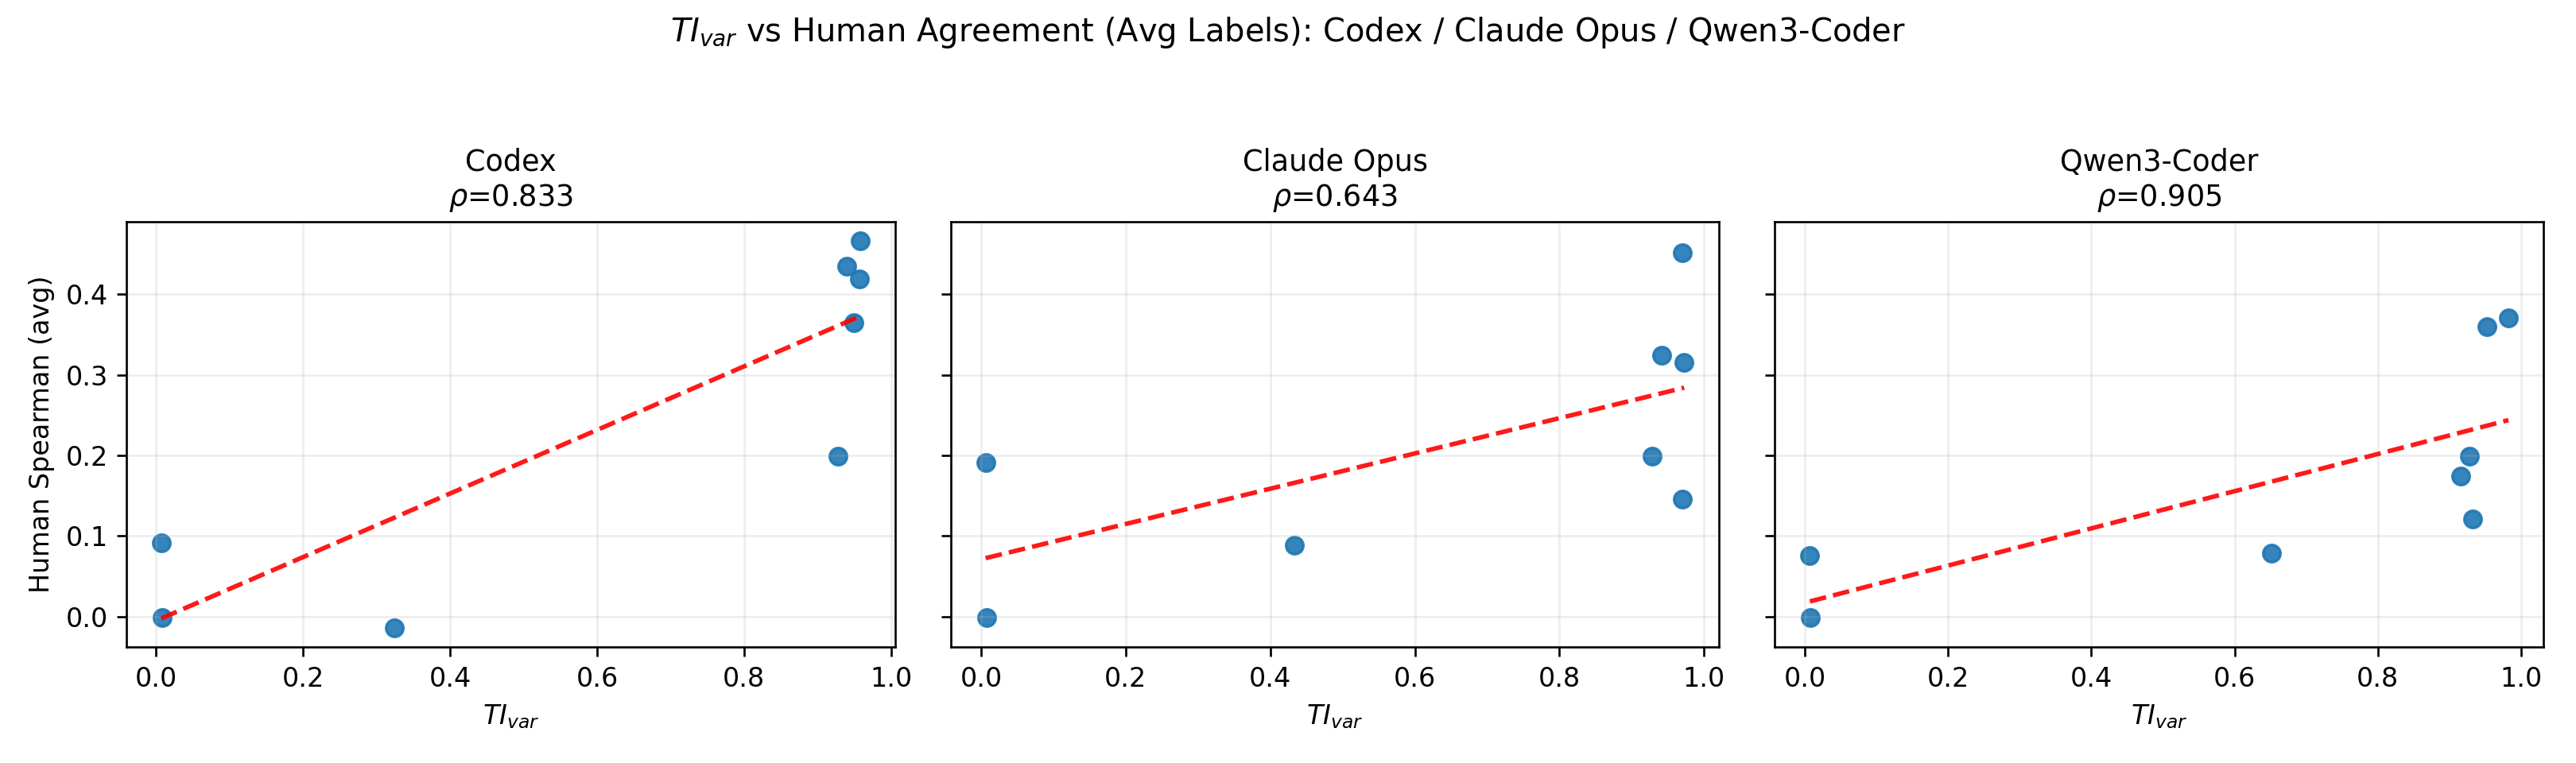
\includegraphics[width=\linewidth]{figures/fig_tivar_scatter_3models_avg.png}
      \caption{Higher \tivar{} $\rightarrow$ higher human agreement in \textbf{all three judge families}.}
    \end{figure}

    \textbf{Catches what agreement misses:} a broken judge hits ${\approx}0.45$ human Spearman yet fails weak monotonicity ($12.5\%$).

  \end{block}

  % CS197 move 5 (stress evidence + honest failure mode + downstream one-liner)
  \vspace{0.6cm}
  \begin{block}{Stress tests keep the judge honest}

    \begin{figure}
      \centering
      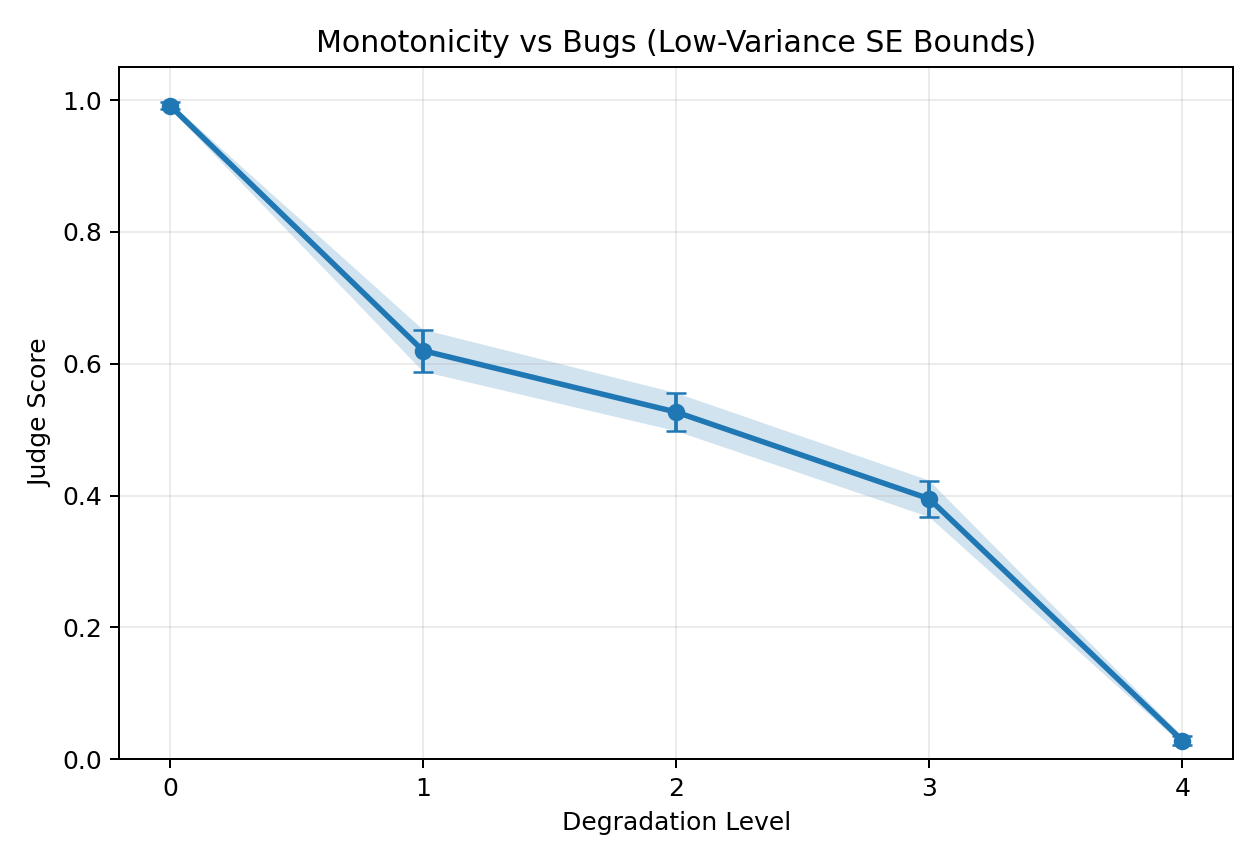
\includegraphics[width=0.49\linewidth]{figures/monotonicity_bugs_lowvar_se_bounds.png}\hfill
      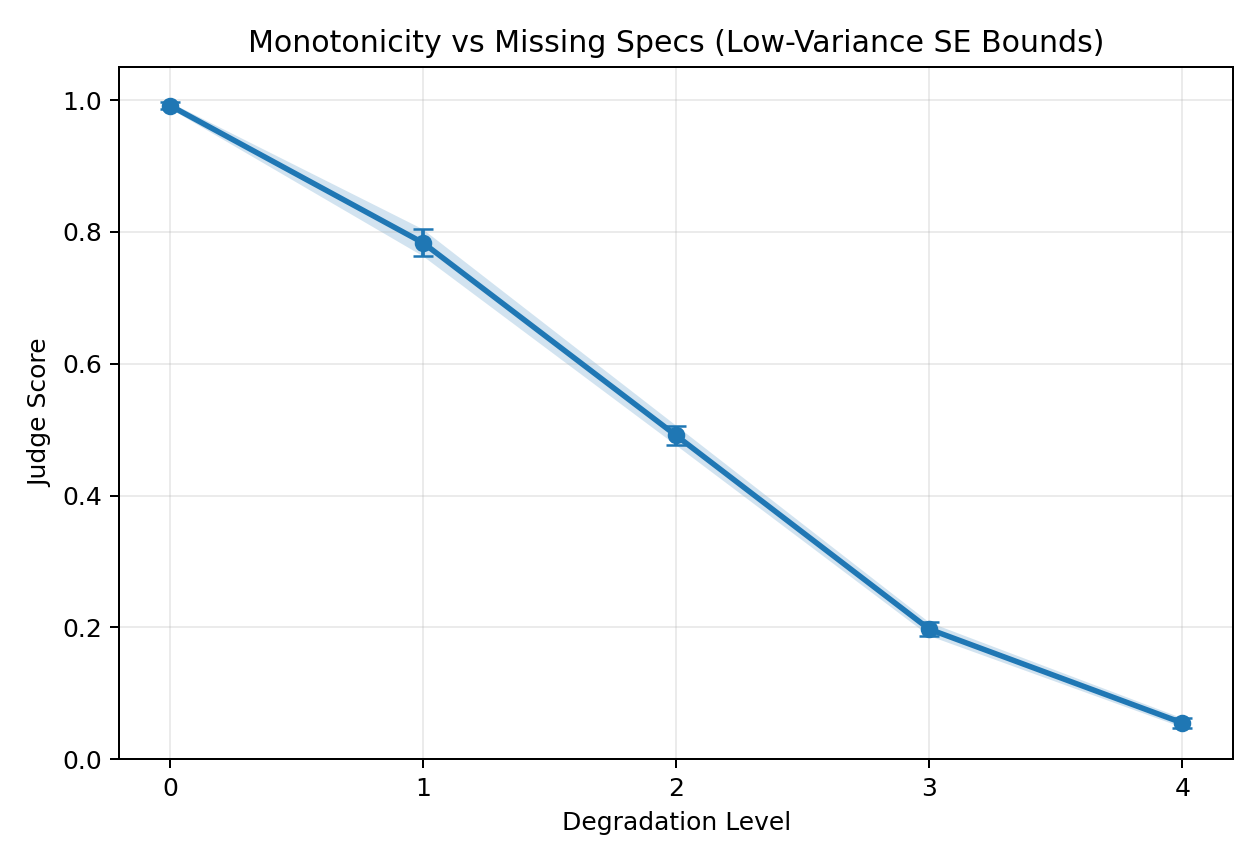
\includegraphics[width=0.49\linewidth]{figures/monotonicity_missing_specs_lowvar_se_bounds.png}
      \caption{GPT-5.3-Codex judge, 184 \textsc{VeriBench} files \cite{mirandaveribench}: scores fall as bugs are injected ($\rho=-0.808$) and as specs are deleted ($\rho=-0.899$).}
    \end{figure}

    \textbf{Known failure mode:} aggressive $\alpha$-renaming scores $0.399$ vs.\ $\geq 0.849$ for milder rewrites.

    \medskip
    Certified judge ranks agents: \textbf{DSPy ReAct 0.615} $>$ Trace++ 0.588 $>$ Trace+ 0.477 $>$ \textbf{baseline 0.470}.

  \end{block}

  % CS197 move 6: takeaways — vision, not self-congratulation; caveat is part of the claim
  \vspace{0.6cm}
  \begin{alertblock}{Takeaways}

    \begin{itemize}
      \setlength{\leftmargini}{2.2em}
      \setlength{\itemsep}{1.2ex}
      \item \textbf{Amortized oversight:} one $n{=}75$ panel + automatic falsifiable checks screen every new judge --- no re-labeling.
      \item \textbf{Measure trust, don't assume it:} behavioral properties expose failures human-agreement scores miss.
      \item \textbf{Scope:} \emph{validation-set calibration evidence, not universal reliability} --- locked held-out test (5 raters, 343 labels, 78 pairs) is next.
    \end{itemize}

  \end{alertblock}

  % QR moved out of the References block to the bottom-right corner (rebalances columns,
  % and puts the scan target where walk-by readers expect it); extra drop so the QR+Code
  % block sits vertically centered on the References block in the left column
  \vspace{2.2cm}
  \bigskip
  {\centering
    \qrcode[height=7cm]{https://github.com/brando90/cert-judge}\\[0.8ex]
    {\small \textbf{Code}}
    % TODO: arXiv link when live
  \par}

\end{column}

\separatorcolumn
\end{columns}
\end{frame}

\end{document}
